% gr-Boolean.tex -- the hypercube Q4 drawn as the lattice of the subsets
% of {a,b,c,d} (Hasse diagram) ; the colour of an edge gives the
% element added. Engine : pdfLaTeX or LuaLaTeX
\documentclass[border=3mm, convert=false]{standalone}
\usepackage{tkz-berge}
\begin{document}
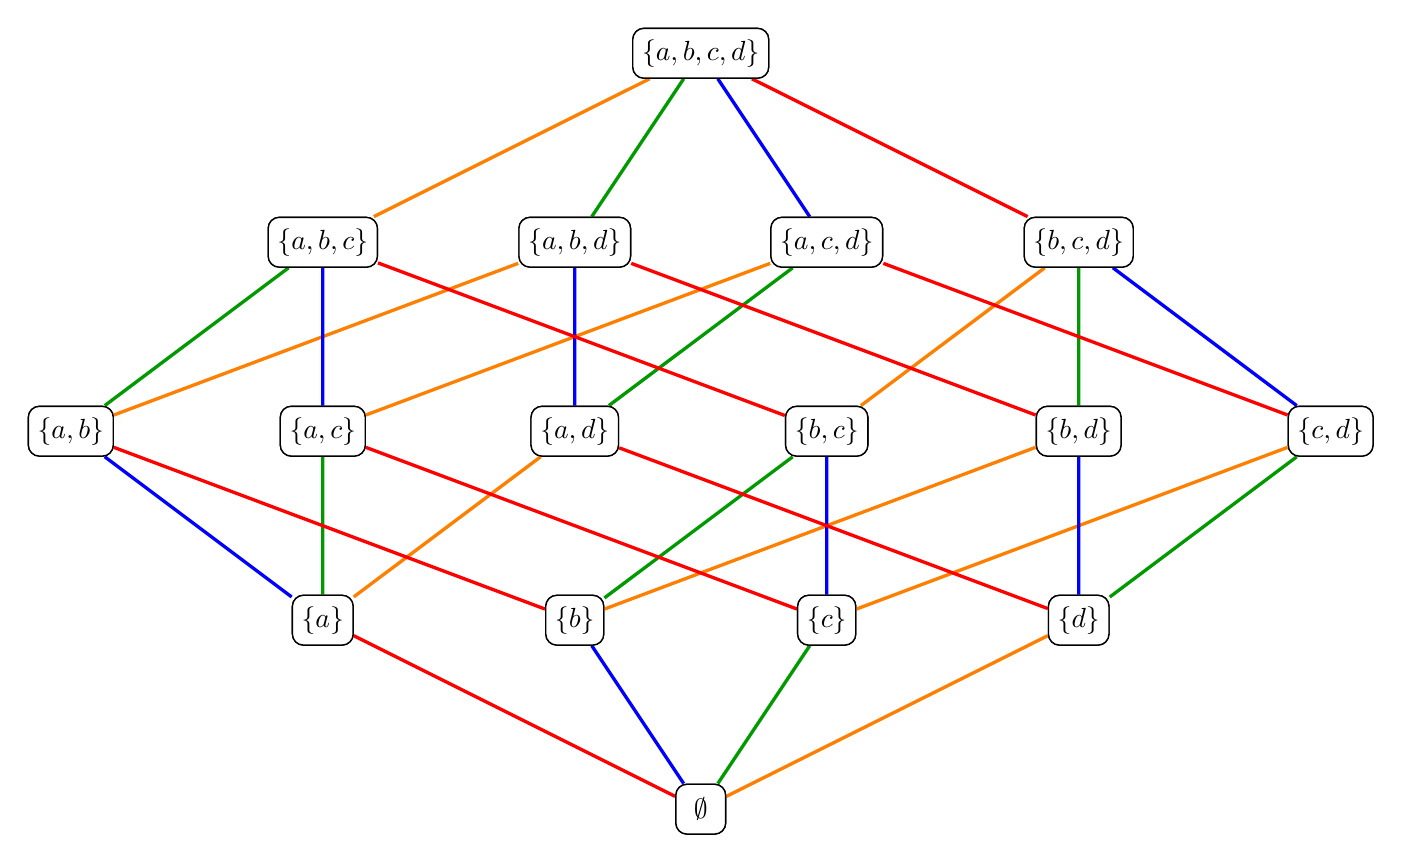
\begin{tikzpicture}[xscale=1.6,yscale=2.4]
  \GraphInit[vstyle=Normal]
  \SetVertexMath
  \tikzset{VertexStyle/.append style = {rectangle, rounded corners,
            minimum size = 18pt, fill = white}}
  % name/x/y/label
  \foreach \n/\x/\y/\l in {
     0/0/0/{\emptyset},
     a/-3/1/{\{a\}}, b/-1/1/{\{b\}}, c/1/1/{\{c\}}, d/3/1/{\{d\}},
     ab/-5/2/{\{a,b\}}, ac/-3/2/{\{a,c\}}, ad/-1/2/{\{a,d\}},
     bc/1/2/{\{b,c\}},  bd/3/2/{\{b,d\}},  cd/5/2/{\{c,d\}},
     abc/-3/3/{\{a,b,c\}}, abd/-1/3/{\{a,b,d\}},
     acd/1/3/{\{a,c,d\}},  bcd/3/3/{\{b,c,d\}},
     abcd/0/4/{\{a,b,c,d\}}}
   {\Vertex[x=\x,y=\y,L=\l]{\n}}
  % the colour gives the element added
  \foreach \s/\t/\c in {
    0/a/red, 0/b/blue, 0/c/green!60!black, 0/d/orange, a/ab/blue,
    a/ac/green!60!black, a/ad/orange, b/ab/red, b/bc/green!60!black,
    b/bd/orange, c/ac/red, c/bc/blue, c/cd/orange, d/ad/red,
    d/bd/blue, d/cd/green!60!black, ab/abc/green!60!black,
    ab/abd/orange, ac/abc/blue, ac/acd/orange, ad/abd/blue,
    ad/acd/green!60!black, bc/abc/red, bc/bcd/orange, bd/abd/red,
    bd/bcd/green!60!black, cd/acd/red, cd/bcd/blue, abc/abcd/orange,
    abd/abcd/green!60!black, acd/abcd/blue, bcd/abcd/red}
    {\Edge[local,color=\c,lw=1.2pt](\s)(\t)}
  \foreach \n/\x/\y/\l in {
     0/0/0/{\emptyset},
     a/-3/1/{\{a\}}, b/-1/1/{\{b\}}, c/1/1/{\{c\}}, d/3/1/{\{d\}},
     ab/-5/2/{\{a,b\}}, ac/-3/2/{\{a,c\}}, ad/-1/2/{\{a,d\}},
     bc/1/2/{\{b,c\}},  bd/3/2/{\{b,d\}},  cd/5/2/{\{c,d\}},
     abc/-3/3/{\{a,b,c\}}, abd/-1/3/{\{a,b,d\}},
     acd/1/3/{\{a,c,d\}},  bcd/3/3/{\{b,c,d\}},
     abcd/0/4/{\{a,b,c,d\}}}
   {\Vertex[x=\x,y=\y,L=\l]{\n}}
\end{tikzpicture}
\end{document}
